%versi 2 (8-10-2016)
\chapter{Landasan Teori}
\label{chap:teori}

\lstdefinelanguage{JavaScript}{
  keywords={new, true, false, function, return, null, catch, switch, var, if, while, do, else, const, this,Math},
  keywordstyle=\color{blue}\bfseries,
  ndkeywords={moveTo,lineTo,arc,random,floor},
  ndkeywordstyle=\color{purple}\bfseries,
  identifierstyle=\color{black},
  sensitive=false,
  comment=[l]{//},
  morecomment=[s]{/*}{*/},
  commentstyle=\itshape\color{green},
  stringstyle=\color{red},
  morestring=[b]',
  morestring=[b]",
  captionpos=b,
}

\lstset{
   language=JavaScript,
   backgroundcolor=\color{white},
   extendedchars=true,
   basicstyle=\fontfamily{fvm}\selectfont\small, 
   showstringspaces=false,
   showspaces=false,
   numbers=left,
   numberstyle=\footnotesize,
   numbersep=5pt,
   tabsize=4,
   breaklines=true,
   showtabs=false,
   captionpos=b,
   frame=leftline,
   stepnumber=1,
   literate={-}{-}1{-\,-}{--}1
}

\section{\textit{Snake}}
\label{sec:snake}
\textit{Snake} merupakan permainan mengendalikan ular untuk mendapatkan makanan yang terdapat pada labirin. Dalam permainan ini, pemain mengendalikan ular untuk mendapatkan makanan sebanyak-banyaknya. Setiap ular memakan makanan, maka skor akan bertambah 1 poin dan tubuh ular akan bertambah panjang. Biasanya makanan hanya ada 1 saja pada sebuah labirin. Ketika makanan itu sudah termakan oleh ular, makanan tersebut akan ditempatkan secara acak. Ular dapat bergerak ke atas, bawah, kiri, dan kanan. Namun pada permainan \textit{Snake} yang akan dibuat sekarang, ular dapat bergerak ke segala arah seperti ilustrasi pada Gambar~\ref{fig:ularSegalaArah}. Permainan akan berakhir jika ular menabrak dinding yang terdapat pada labirin atau ular tersebut menabrak tubuhnya sendiri. \\

\begin{figure}[H]
	\centering  
	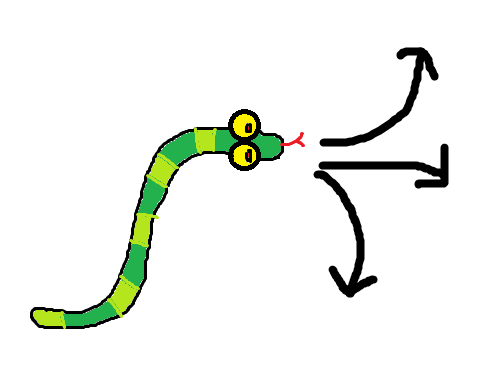
\includegraphics[scale=0.4]{ular-segala-arah}  
	\caption[Pergerakan ular ke segala arah]{Pergerakan ular ke segala arah} 
	\label{fig:ularSegalaArah} 
\end{figure} 

Permainan \textit{Snake} ini dapat dimainkan secara \textit{singleplayer} atau \textit{multiplayer}. \textit{Singleplayer game} adalah permainan yang dapat dimainkan oleh 1 pemain. \textit{Multiplayer game} adalah permainan yang dapat dimainkan oleh beberapa pemain. Pada umumnya, permainan \textit{Snake} dimainkan secara \textit{singleplayer}. Contoh \textit{singleplayer game Snake} adalah \textit{Snake} pada telepon genggam \textit{Nokia} yang dapat dilihat pada Gambar~\ref{fig:nokiaSnake}\footnote{https://en.wikipedia.org/wiki/Snake\_(video\_game\_genre)} dan contoh \textit{multiplayer game Snake} adalah \textit{Slither.io} yang dapat dilihat Gambar~\ref{fig:slither}\footnote{https://play.google.com/store/apps/details?id=air.com.hypah.io.slither}. \textit{Snake} dapat dimainkan menggunakan \textit{smartphone} dan \textit{web browser}.  

\begin{figure}[H]
	\centering  
	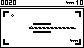
\includegraphics[scale=2]{nokiaSnake}  
	\caption[Permainan Snake pada telepon genggam \textit{Nokia}]{Permainan Snake pada telepon genggam \textit{Nokia}} 
	\label{fig:nokiaSnake} 
\end{figure} 

\begin{figure}[H]
	\centering  
	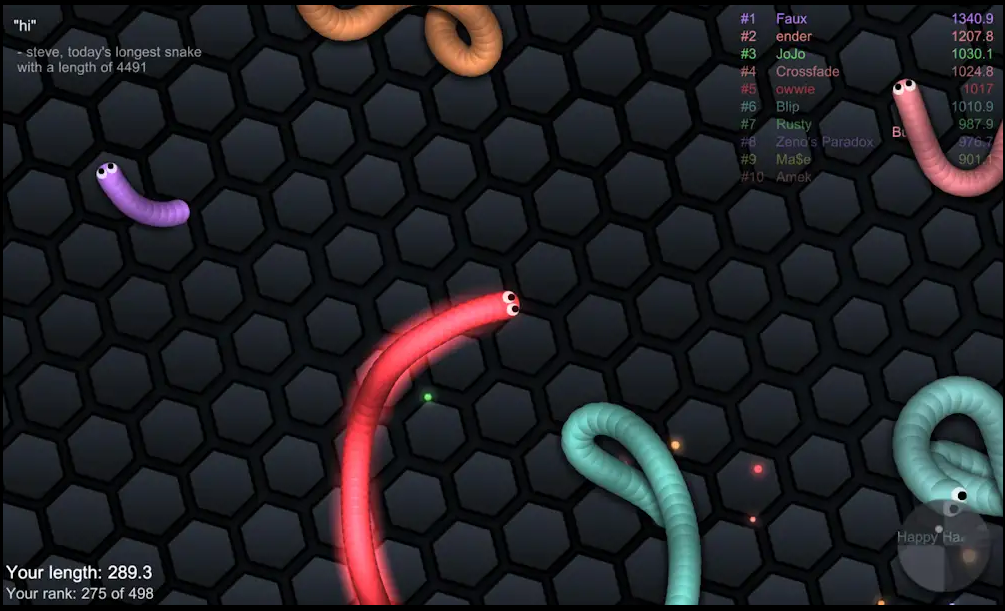
\includegraphics[scale=0.3]{slither}  
	\caption[Permainan \textit{Slither.io} pada \textit{Android}]{Permainan \textit{Slither.io} pada \textit{Android}} 
	\label{fig:slither} 
\end{figure} 

\section{HTML5 \textit{Canvas}}
\label{sec:HTML5Canvas}
HTML5 Canvas adalah sebuah daerah \textit{bitmap} yang dapat dimanipulasi oleh \textit{Javascript}. Pada daerah \textit{bitmap} tersebut, \textit{pixel-pixel} akan di\textit{render} oleh canvas. Setiap \textit{frame}, HTML5 Canvas akan menggambar pada area \textit{bitmap} tersebut menggunakan \textit{Canvas} API(\textit{Application Programming Interface}) yang dipanggil pada \textit{Javascript}. API dari HTML5 Canvas yang umum adalah 2D \textit{Context}. Dengan adanya 2D \textit{Context}, \textit{programmer} dapat membuat bentuk 2D, menampilkan gambar, \textit{render} tulisan, memberi warna, membuat garis dan kurva, dan manipulasi \textit{pixel}. HTML5 Canvas tidak hanya digunakan untuk menggambar dan menampilkan gambar serta tulisan. HTML5 Canvas dapat digunakan untuk membuat animasi, aplikasi pada \textit{web} dan permainan. 

Untuk menambahkan \textit{canvas} pada halaman HTML, diperlukan \textit{tag} <canvas>. Di bawah ini adalah potongan kode untuk menambahkan \textit{canvas} pada halaman HTML. 

\begin{lstlisting}[language=HTML, caption=Menambahkan \textit{canvas}]
	<canvas id='canvas' width='500' height='300'>
		Your browser does not support HTML5 Canvas.
	</canvas>
	
\end{lstlisting}


Berikut adalah penjelsan atribut yang ada pada \textit{canvas} berdasarkan potongan kode di atas : 
\begin{itemize}
	\item id
\end{itemize}


\section{\textit{\textit{Javascript}}}
\label{sec:Javascript}
\textit{Javascript} adalah bahasa pemrograman yang ringan, \textit{interpreted} dan berorientasi objek yang digunakan pada halaman \textit{web}. \textit{Javascript} dapat membuat objek dengan menambahkan \textit{method} dan atributnya sama seperti bahasa pemrograman C++ dan \textit{Java}. Setelah objek diinisialisasi, maka objek tersebut dapat dijadikan \textit{blueprint} untuk membuat objek lain yang mirip\footnote{https://developer.mozilla.org/en-US/docs/Web/JavaScript/About\_JavaScript}. \textit{Javascript} dapat digunakan untuk mengimplementasi hal yang kompleks pada halaman web. Contohnya adalah menamplikan peta yang interaktif dan membuat animasi 2D/3D. Selain \textit{Javascript}, HTML(\textit{HyperText Markup Language}) dan CSS(\textit{Cascading Style Sheet}) merupakan bagian/komponen penting dalam pembuatan halaman \textit{web}\footnote{https://developer.mozilla.org/en-US/docs/Learn/JavaScript/First\_steps/What\_is\_JavaScript}.\\

Untuk menambahkan Javascript pada sebuah halaman web yang dibuat, gunakan tag <script>. Ada 2 cara untuk menambahkan Javascript yaitu menambahkan langsung di halaman web tersebut(Internal Javascript) dan menambahkan file Javascript terpisah(External Javascript).

\subsection{Variabel}
Variabel adalah sebuah wadah untuk menyimpan nilai/\textit{value}. Untuk mendeklarasi variable pada \textit{Javascript}, digunakan \textit{keyword 'var'}. Variabel pada Javascript tidak perlu menuliskan tipe datanya ketika mendeklarasikan variabel. Di bawah ini adalah potongan kode untuk mendeklarasikan variabel.\footnote{https://developer.mozilla.org/en-US/docs/Web/JavaScript/Guide/Grammar\_and\_types}

\begin{lstlisting}[language=Javascript, caption=Deklarasi variabel]
	var myVariable;
	
\end{lstlisting}

Nilai variabel pada potongan kode di atas adalah \textit{undifined} karena variabel tersebut tidak diberi nilai/value. Di bawah ini adalah potongan kode untuk mengisi nilai pada variabel. 

\begin{lstlisting}[language=Javascript, caption=Mengisi nilai sebuah variabel]
	myVariable = 3;	
	
\end{lstlisting}

Variabel dapat menyimpan beberapa tipe data diantaranya adalah\footnote{https://developer.mozilla.org/en-US/docs/Learn/Getting\_started\_with\_the\_web/JavaScript\_basics} :
\begin{itemize}
	\item \textit{String} : nilai yang berupa teks atau sekumpulan huruf.
	\item \textit{Number} : nilai yang berupa angka.
	\item \textit{Boolean} : nilai \textit{true/false}.
	\item \textit{Array} : struktur untuk menyimpan lebih dari 1 nilai dalam sebuah \textit{reference}
	\item \textit{Object} : semua yang ada pada Javascript termasuk objek pada HTML.
\end{itemize}

\subsection{\textit{Constant}}
\textit{Constant} adalah sebuah variabel \textit{read-only}, artinya nilai pada \textit{constant} tidak dapat diubah. Untuk mendeklarasikan \textit{constant}, digunakan \textit{keyword 'const'}. Di bawah ini adalah potongan kode untuk mendeklarasi \textit{constant}.

\begin{lstlisting}[language=Javascript, caption=Deklarasi \textit{constant}]
	const myConst = 1;
	
\end{lstlisting}

\subsection{\textit{Function}}
\textit{Function} adalah sekumpulan perintah/\textit{statements} untuk menjalankan suatu tugas atau menghitung nilai. Untuk membuat \textit{function}, digunakan \textit{keyword 'function'}, kemudian diikuti dengan nama \textit{function} tersebut, parameter yang dituliskan di dalam kurung, dan \textit{statement}/perintah \textit{Javascript} yang ditulis di dalam kurung kurawal. Parameter pada \textit{function} bisa lebih dari 1 yang penulisanya dipisahkan oleh tanda koma (,). \textit{Function} bisa memiliki parameter atau tidak. Di bawah ini adalah potongan kode untuk membuat \textit{function} penjumlahan 2 buah bilangan.

\begin{lstlisting}[language=Javascript, caption=\textit{Function} penjumlahan 2 buah bilangan]
	function penjumlahan(angka1,angka2){
		var hasil = angka1+angka2;
		return hasil;
	}
	
\end{lstlisting}

Setelah membuat \textit{function}, \textit{function} tersebut tidak langsung dieksekusi. Membuat \textit{function} hanya memberi nama \textit{function} tersebut dan mendeskripsikan apa yang akan dilakukan oleh \textit{function} tersebut apabila dipanggil. Dengan memanggil \textit{function}, maka \textit{function} akan dieksekusi\footnote{https://developer.mozilla.org/en-US/docs/Web/JavaScript/Guide/Functions}. Di bawah ini adalah potongan kode untuk memanggil \textit{function} dengan nama penjumlahan.

\begin{lstlisting}[language=Javascript, caption=Memanggil \textit{function} penjumlahan]
	penjumlahan(10,5);
	
\end{lstlisting}

\subsection{Menggambar pada \textit{Canvas}}
Sesudah menuliskan \textit{tag} <canvas> pada HTML, canvas tidak bisa langsung digambar. Karena itu perlu ditambahkan \textit{drawing context} pada \textit{Javascript}. Di bawah ini adalah potongan kode untuk menambahkan \textit{drawing context}.

\begin{lstlisting}[language=Javascript, caption=Menambahkan \textit{drawing context canvas}]
	var myCanvas = document.getElementById('canvas');
	var context = myCanvas.getContext('2d');
\end{lstlisting}

Berdasarkan potongan kode di atas, variabel myCanvas menyimpan objek dengan id = 'canvas'. Id ini mengacu ke objek \textit{canvas} pada HTML yang memilki id bernama canvas. Variabel myCanvas sekarang sudah menyimpan objek \textit{canvas}. Kemudian variabel context menyimpan \textit{drawing context} 2D. Sesudah itu, \textit{canvas} tersebut dapat digambar dengan bentuk 2D, garis, kurva, membuat tulisan, dan menambahkan gambar. Selain untuk menggambar, bentuk-bentuk tersebut dapat diberi warna sesuai dengan keinginan.\\

Untuk menggambar bentuk 2D atau garis, diperlukan koordinat x dan y. Koordinat tersebut akan menempatkan gambar tersebut pada \textit{canvas}. Posisi awal/\textit{origin} pada \textit{canvas} adalah (0,0) yang terletak di ujung kiri atas \textit{canvas}. Gambar~\ref{fig:grid}\footnote{https://developer.mozilla.org/en-US/docs/Web/API/Canvas\_API/Tutorial/Drawing\_shapes} adalah penempatan kotak biru pada \textit{canvas} terhadap \textit{origin}.

\begin{figure}[H]
	\centering  
	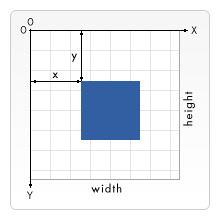
\includegraphics[scale=0.7]{grid}
	\caption[Posisi kotak biru pada \textit{canvas} terhadap \textit{origin}]{Posisi kotak biru pada \textit{canvas} terhadap \textit{origin}}
	\label{fig:grid} 
\end{figure} 

Pada di atas, titik ujung kiri kotak biru tersebut berjarak x \textit{pixel} dari kiri dan berjarak y \textit{pixel} dari atas. 

\subsubsection{Menggambar Persegi Panjang}
Ada 3 cara untuk menggambar persegi panjang:

\begin{itemize}
	\item \textit{fillRect(x,y,width,height)} : menggambar persegi panjang serta mengisi bagian tengah persegi panjang.
	\item \textit{strokeRect(x,y,width,height)} : menggambar \textit{outline} yang berbentuk persegi panjang.
	\item \textit{clearRect(x,y,width,height)} : menghapus daerah yang ditentukan pada \textit{canvas}. Daerah yang dihapus berbentuk persegi panjang.
	\item \textit{rect(x,y,width,height)} : menambah \textit{path} berbentuk persegi panjang.
\end{itemize}

Fungsi tersebut memiliki parameter yang sama. Parameter x dan y untuk menentukan posisi pada canvas dari titik ujung kiri atas persegi panjang. \textit{Width} adalah lebar dari persegi panjang dan \textit{height} adalah tinggi dari persegi panjang.

\subsubsection{Menggambar \textit{Path}}
\textit{Path} adalah sekumpulan titik yang dihubungkan oleh segmen garis. \textit{Path} dapat membentuk kurva dan membuat bentuk 2D lainnya seperti segitiga, trapesium, belah ketupat dan lain-lain. Langkah-langkah untuk membuat bentuk menggunakan path adalah sebegai berikut : 

\begin{enumerate}
	\item Buat \textit{path}.
	\item Tuliskan perintah untuk menggambar pada \textit{path} tersebut.
	\item Sesudah \textit{path} tersebut sudah dibuat, \textit{path} tersebut dapat di\textit{render} menggunakan \textit{stroke} atau \textit{fill}.
\end{enumerate}

Langkah pertama untuk membuat \textit{path} baru adalah dengan menggunakan fungsi \textit{beginPath()}. Setelah itu, perintah-perintah untuk menggambar dapat digunakan untuk membuat bentuk-bentuk yang diinginkan. Apabila sudah selesai menggambar, gunakan fungsi \textit{stroke()} untuk menggambar outline dari \textit{path} tersebut atau \textit{fill()} untuk mengisi area path tersebut. Setelah itu, gunakan fungsi \textit{closePath()} untuk menutup bentuk tersebut dengan cara menggambar garis lurus dari posisi titik terakhir ke titik awal. Fungsi lainnya yang menjadi bagian dari membuat \textit{path} adalah fungsi \textit{moveTo()}. Fungsi ini diibaratkan seperti mengangkat sebuah pensil dari sebuah titik pada kertas kemudian menempatkanya pada titik yang diinginkan. Di bawah ini adalah fungsi \textit{moveTo()}.

\begin{lstlisting}[language=Javascript, caption=Fungsi \textit{moveTo()}]
	moveTo(x,y);
\end{lstlisting}

Fungsi \textit{moveTo()} memiliki 2 parameter yaitu x dan y yang merupakan posisi titik pada \textit{canvas}. Ketika canvas sudah diinisialsasi dan fungsi \textit{beginPath()} sudah dipanggil, fungsi \textit{moveTo()} berguna sebagai penempatan titik awal untuk menggambar. Fungsi \textit{lineTo()} digunakan untuk menggambar sebuah garis. Di bawah ini adalah fungsi \textit{lineTo()}.

\begin{lstlisting}[language=Javascript, caption=Fungsi \textit{lineTo()}]
	lineTo(x,y);
\end{lstlisting}

Fungsi \textit{lineTo()} memiliki 2 parameter yaitu x dan y yang merupakan titik akhir dari garis. Garis akan digambar mulai dari posisi titik awal sampai ke posisi titik akhir garis. Titik awal ini bergantung pada titik akhir dari \textit{path} sebelumya. Titik awal dapat diubah dengan menggunakan fungsi \textit{moveTo()}.

Fungsi \textit{arc()} digunakan untuk menggambar lingkaran atau busur. Di bawah ini adalah fungsi arc().

\begin{lstlisting}[language=Javascript, caption=Fungsi \textit{arc()}]
	arc(x,y,radius,startAngle,endAngle,anticlockwise);
\end{lstlisting}

Parameter x dan y adalah posisi titik tengah busur pada canvas. Radius adalah besar jari-jari busur. StartAngle dan endAngle adalah titik awal dan titik akhir busur dalam satuan radian yang diukur dari sumbu x. Anticlockwise adalah parameter yang bernilai boolean, apabila bernilai true, maka busur akan digambar berlawanan arah jarum jam dan jika bernilai false, busur akan digambar searah jarum jam. Karena fungsi arc() menerima input sudut dalam radian, maka perlu dilakukan konversi dari satuan derajat menjadi radian terlebih dahulu. Rumusnya adalah sebagai berikut :

\begin{displaymath}
	radian = (Math.PI / 180) * besar sudut
\end{displaymath}	

\textit{B\'ezier curve} merupakan tipe \textit{path} yang digunakan untuk membuat kurva. \textit{B\'ezier curve} ada 2 jenis yaitu \textit{cubic} dan \textit{quadratic}. Perbedaanya adalah \textit{quadratic B\'ezier curve} memiliki sebuah \textit{control point}, sedangkan \textit{cubic B\'ezier curve} memiliki 2 buah \textit{control point}. Pada Gambar~\ref{fig:bezier}\footnote{https://developer.mozilla.org/en-US/docs/Web/API/Canvas\_API/Tutorial/Drawing\_shapes} menunjukkan perbedaan antara \textit{quadratic B\'ezier curve} dan \textit{cubic B\'ezier curve}. Titik merah pada gambar merupakan \textit{control point} dari \textit{B\'ezier curve}.

\begin{figure}[H]
	\centering  
	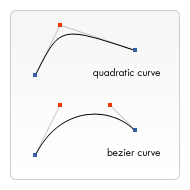
\includegraphics[scale=1]{bezier}
	\caption[Perbedaan \textit{quadratic B\'ezier curve} dan \textit{cubic B\'ezier curve}]{Perbedaan \textit{quadratic B\'ezier curve} dan \textit{cubic B\'ezier curve}}
	\label{fig:bezier} 
\end{figure} 

Berikut adalah fungsi \textit{quadratic} dan \textit{cubic B\'ezier curve} :
\begin{itemize}
	\item \textit{quadraticCurveTo(cp1,cp2,x,y)} : menggambar \textit{quadratic B\'ezier curve} dari posisi pensil sekarang ke titik akhir yaitu x dan y, dengan titik control point yaitu cp1 dan cp2.
	\item bezierCurveTo(cp1x,cp1y,cp2x,cp2y,x,y) : menggambar \textit{cubic B\'ezier curve} dari posisi pensil sekarang ke titik akhir yaitu x dan y, dengan 2 titik control point yaitu (cp1x,cp1y) dan (cp2x,cp2y).
\end{itemize}

\subsection{\textit{Object Oriented Programming Javascript}}
OOP (\textit{Object Oriented Programming}) adalah sebuah paradigma \textit{programming} yang menggunakan abstraksi untuk membuat objek-objek yang ada pada dunia nyata. Bahasa pemrograman seperti \textit{Java}, C++, \textit{Ruby, Phyton}, PHP, dan \textit{Objective-C} sudah mendukung OOP. Dalam OOP, setiap objek dapat menerima pesan, memproses data dan mengirim pesan ke objek lain. Program yang menggunakan konsep OOP ini mudah untuk dimengerti dan lebih mudah untuk dikembangkan oleh \textit{programmer}\footnote{https://developer.mozilla.org/ms/docs/Web/JavaScript/Introduction\_to\_Object-Oriented\_JavaScript}. \\

Ide umum pada OOP adalah menggunakan objek untuk memodelkan benda-benda yang ada pada dunia nyata. Objek tersebut kemudian direpresentasi pada program yang dibuat. Objek-objek dapat berisi data, fungsionalitas dan \textit{behaviour} yang merepresentasikan informasi tentang objek tersebut dan tugas objek\footnote{https://developer.mozilla.org/en-US/docs/Learn/JavaScript/Objects/Object-oriented\_JS}. Contohnya, bila ingin membuat objek sebuah mobil. Mobil memiliki beberapa informasi diantaranya adalah merk mobil, berat mobil, warna mobil dan tahun produksi. Informasi tersebut dapat disebut sebagai properti dari objek. Mobil dapat bergerak maju, berbelok ke kanan, berbelok ke kiri, bergerak mundur dan berhenti. Hal-hal yang dapat dilakukan oleh objek disebut sebagai method dari objek. 

\subsubsection{Kelas}
\textit{Javascript} tidak memiliki \textit{statement 'class'} yang dapat digunakan pada bahasa pemrograman C++ atau \textit{Java}. Untuk membuat kelas, \textit{Javascript} menggunakan \textit{function} sebagai konstruktor untuk kelas. Karena itu, membuat kelas sama dengan membuat \textit{function} pada \textit{Javascript}. Di bawah ini adalah potongan kode untuk membuat kelas bernama Mobil.

\begin{lstlisting}[language=Javascript, caption=Membuat kelas Mobil]
	function Mobil(){
	
	}
	
\end{lstlisting}

\subsubsection{Objek}
Untuk membuat instansi baru dari objek, gunakan \textit{statement 'new'} yang nantinya akan disimpan pada variabel. Di bawah ini adalah potongan kode untuk membuat instansi.

\begin{lstlisting}[language=Javascript, caption=Membuat \textit{instance} mobil]
	var mobil1 = new Mobil();
\end{lstlisting}

\subsubsection{Konstruktor}
Konstruktor adalah \textit{method} yang ada pada kelas. Konstruktor akan dipanggil ketika pertama kali inisialisasi atau saat instansi baru dari objek dibuat. \textit{Function} pada \textit{Javascript} berfungsi sebagai konstruktor sehingga tidak perlu membuat method konstruktor lagi. Semua aksi yang terdapat pada kelas akan dieksekusi pada saat instansiasi.

\subsubsection{Properti/Atribut}
Properti adalah variabel yang terdapat pada kelas. Properti ditulis pada konstruktor kelas sehingga setiap properti pada kelas akan dibuat ketika membuat instansi baru. Untuk membuat properti, gunakan \textit{statement 'this'}. Cara ini mirip dengan bahasa pemrograman \textit{Java} ketika membuat sebuah properti pada objek. Sintaks untuk mengakses properti di luar kelas adalah : namaInstansi.properti. Di bawah ini adalah potongan kode untuk mendefinisikan properti pada kelas Mobil pada saat instansiasi.

\begin{lstlisting}[language=Javascript, caption=Mendefinisikan properti pada kelas Mobil]
	function Mobil(merkMobil,beratMobil,warnaMobil,tahunProduksi){
		this.merkMobil = merkMobil;
		this.beratMobil = beratMobil; //satuan dalam kg
		this.warnaMobil = warnaMobil;
		this.tahunProduksi = tahunProduksi;
	}
	
	var mobil1 = new Mobil('Toyota',1000,'Hitam',2010);
	
\end{lstlisting}

\subsubsection{\textit{Method}}
\textit{Method} adalah hal yang dapat dilakukan oleh sebuah objek. Untuk membuat \textit{method}, tuliskan nama \textit{method} terlebih dahulu kemudian \textit{assign} fungsi pada nama method tersebut. Untuk memanggil \textit{method} sebuah objek, tuliskan nama objek/kelas terlebih dahulu, kemudian tuliskan nama \textit{method} sesuai dengan yang sudah dibuat beserta tanda kurung. Tanda kurung berisi parameter. Di bawah ini adalah potongan kode untuk membuat dan memanggil method bergerakMaju() pada kelas Mobil.

\begin{lstlisting}[language=Javascript, caption=Membuat dan memanggil method bergerakMaju()]
	function Mobil(merkMobil,beratMobil,warnaMobil,tahunProduksi){
		this.merkMobil = merkMobil;
		this.beratMobil = beratMobil; //satuan dalam kg
		this.warnaMobil = warnaMobil;
		this.tahunProduksi = tahunProduksi;
		
		this.bergerakMaju = function(){
			//kode agar mobil bergerak maju
		}
	}
	
	var mobil1 = new Mobil('Toyota',1000,'Hitam',2010);
	mobil1.bergerakMaju(); //memanggil fungsi untuk bergerak maju
	
\end{lstlisting}

\subsection{\textit{Event}}
\textit{Event} adalah kejadian/peristiwa yang terjadi pada sistem yang diprogram. Sistem akan memberitahu apabila kejadian tersebut sudah terjadi dan akan melakukan suatu aksi ketika kejadian sudah terjadi. Misalnya, di bandara ketika landasan pacu sudah bersih untuk pesawat lepas landas, sinyal akan dikomunikasikan kepada pilot bahwa pesawat sudah boleh untuk lepas landas. Dalam \textit{web}, \textit{event} ditembakan di dalam \textit{browser window} dan dikaitkan pada objek yang spesifik seperti sekumpulan elemen, dokumen HTML yang dimuat atau keseluruhan \textit{browser window}. Ada beberapa \textit{event} yang dapat terjadi diantaranya adalah : 

\begin{itemize}
	\item Pengguna mengklik sebuah element atau mengarahkan kursor ke sebuah elemen.
	\item Pengguna menekan sebuah tombol pada \textit{keyboard}.
	\item Pengguna mengatur besar dan menutup \textit{browser window}.
	\item Halaman \textit{web} selesai dimuat.
	\item \textit{Form} sedang di\textit{submit}.
	\item Video sedang dimainkan, dijeda, atau selesai.
	\item Ketika \textit{error} terjadi.
\end{itemize}

Setiap \textit{event} memiliki \textit{event handler}, yang berisikan sekumpulan kode yang akan dijalankan ketika \textit{event} sudah terjadi. \textit{Event handler} juga sering disebut sebagai \textit{event listener}. \textit{Listener} menunggu \textit{event} yang terjadi dan \textit{handler} adalah kode yang dijalankan ketika \textit{listener} mendapatkan \textit{event}/ketika \textit{event} terjadi. Untuk memperjelas bagaimana cara menggunakan \textit{event}, di bawah ini terdapat contoh kode untuk menambahkan event pada button/tombol.

\begin{lstlisting}[language=Javascript,{alsolanguage=HTML}, caption=Menambahkan event pada button]
	<html>
		<title>Event pada tombol</title>
		<body>
			<button id='tombol'>Change color</button>
		</body>
	</html>
	
	<script>
		var btn = document.getElementById('tombol');

		function random(number) {
  			return Math.floor(Math.random()*(number+1));
		}

		btn.onclick = function() {
  			var rndCol = 'rgb(' + random(255) + ',' + random(255) + ',' + random(255) + ')';
  			document.body.style.backgroundColor = rndCol;
		}
	</script>
	
\end{lstlisting}

Berdasarkan kode di atas, objek \textit{button} dengan id='tombol' disimpan di dalam variabel bernama 'btn'. Ada fungsi bernama \textit{'random'} untuk mengembalikan sebuah nilai acak. Setelah itu ada \textit{event handler}. \textit{Event handler property} yang digunakan adalah \textit{onclick}. \textit{Event handler property onclick} mengecek apakah objek(dalam kasus ini objeknya adalah button) sudah ditekan/diklik. Bila tombol sudsh diklik, maka akan mengeksekusi fungsi untuk mengubah warna \textit{background}. Warna RGB tersebut di\textit{generate} secara acak menggunakan fungsi \textit{random} yang sudah dibuat sebelumnya. Tidak hanya \textit{event handler property onclick} saja yang dapat digunakan pada halaman web. Berikut ini adalah beberapa \textit{event handler property} lainnya:

\begin{itemize}
	\item \textit{onfocus} dan \textit{onblur} : event akan terjadi apabila sebuah objek difokuskan/tidak. Biasanya digunakan untuk menampilkan informasi tentang bagaimana cara mengisi \textit{form} ketika difokuskan atau menampilkan pesan \textit{error} ketika \textit{form} tersebut diisi dengan nilai yang salah/tidak valid.
	\item \textit{ondblclick} : \textit{event} akan terjadi ketika objek diklik 2 kali/\textit{double click}.
	\item \textit{window.keypress, window.onkeydown, window.onkeyup} : \textit{event} akan terjadi apabila sebuah tombol pada \textit{keyboard} ditekan. \textit{Keypress} adalah \textit{event} ketika tombol ditekan kemudian dilepas. \textit{Keydown} adalah \textit{event} ketika tombol ditekan dan \textit{keyup} adalah \textit{event} ketika tombol dalam keadaan tidak ditekan. Untuk ketiga \textit{event} ini, event tersebut harus di\textit{register} pada objek \textit{window} yang merepresentasikan \textit{browser window}.
	\item \textit{onmouseover} dan \textit{onmouseout} : event akan terjadi ketika posisi kursor \textit{mouse} berada luar objek lalu ditempatkan di atas objek dan ketika posisi kursor \textit{mouse} berada di atas objek lalu keluar dari objek. 
\end{itemize}

Beberapa \textit{event handler property} tersebut sangat umum dan tersedia di manapun, sedangkan beberapa \textit{event handler property} lainnya sangat spesifik dan hanya digunakan untuk elemen tertentu, contohnya adalah menggunakan \textit{onplay} untuk elemen tertentu yaitu <video>.\\

Mekanisme event terbaru dalam spesifikasi DOM(\textit{Document Object Model}) \textit{level} 2 \textit{Events} yang memberikan \textit{browser} sebuah fungsi baru yaitu \textit{addEventListener()}. Fungsi ini mirip seperti \textit{event handler property} namun memiliki sintaks yang berbeda. Di bawah ini adalah potongan kode untuk menggunakan fungsi \textit{addEventListener()}.

\begin{lstlisting}[language=Javascript, caption=Menggunakan fungsi addEventListener()]

	var btn = document.getElementById('tombol');

	function bgChange() {
  		var rndCol = 'rgb(' + random(255) + ',' + random(255) + ',' + random(255) + ')';
  		document.body.style.backgroundColor = rndCol;
	}   

	btn.addEventListener('click', bgChange);
	
\end{lstlisting}

Pada fungsi \textit{addEventListener()}, ada 2 buah parameter yaitu \textit{event} yang ingin digunakan(dalam potongan kode di atas menggunakan \textit{event click}) dan kode sebagai \textit{handler} yang ingin dijalankan ketika \textit{event} tersebut terjadi. Selain cara di atas, dapat juga menuliskan semua kode di dalam fungsi \textit{addEventListener()} seperti potongan kode di bawah ini.

\begin{lstlisting}[language=Javascript, caption=Menuliskan kode di dalam fungsi addEventListener()]

	btn.addEventListener('click', function() {
  		var rndCol = 'rgb(' + random(255) + ',' + random(255) + ',' + random(255) + ')';
  		document.body.style.backgroundColor = rndCol;
	});
	
\end{lstlisting}


\subsection{Membuat Animasi}
Ketika menggambar sebuah bentuk pada \textit{canvas}, bentuk tersebut tidak berpindah tempat. Agar bentuk dapat bergerak, bentuk tersebut harus digambar ulang dan semua yang sudah digambar sebelumnya. Langkah-langkah untuk membuat animasi adalah sebagai berikut :

\begin{enumerate}
	\item Membersihkan \textit{canvas} : hilangkan semua bentuk-bentuk yang sudah tergambar di canvas. Untuk menghapus keseluruhan \textit{canvas}, gunakan fungsi \textit{clearRect()}.
	\item Menyimpan \textit{state canvas} : ketika mengubah atribut(seperti \textit{style}) yang mempengaruhi \textit{state canvas} dan ingin \textit{original state} tersebut digunakan kembali, \textit{state} tersebut harus disimpan. 
	\item Gambar bentuk : gambar bentuk yang ingin dianimasikan.
	\item Mengembalikan \textit{state canvas} : jika state sudah disimpan, kembalikan \textit{state} tersebut sebelum menggambar di \textit{frame} yang baru.
\end{enumerate}

Bentuk yang digambar pada \textit{canvas} dapat menggunakan fungsi yang dimiliki oleh \textit{canvas} atau dengan membuat fungsi sendiri. Hasil yang ada pada \textit{canvas} akan muncul setelah \textit{script} selesai mengeksekusi. Jadi dibutuhkan cara untuk mengeksekusi fungsi untuk menggambar dalam waktu tertentu. Ada 3 fungsi yang dapat digunakan untuk memanggil fungsi dalam kurun waktu tertentu diantaranya adalah :

\begin{itemize}
	\item \textit{setInterval(function,delay)}: mengeksekusi fungsi \textit{function} berulang kali setiap \textit{delay} milidetik.
	\item \textit{setTimeout(function,delay)}: mengeksekusi fungsi \textit{function} setiap \textit{delay} milidetik.
	\item \textit{requestAnimationFrame(callback)}: memberitahu \textit{browser} untuk menjalankan animasi dan meminta \textit{browser} memanggil fungsi yang spesifik untuk memperbarui animasi.
\end{itemize}

Jika tidak ingin ada iteraksi user, gunakan fungsi \textit{setInterval()} untuk mengeksekusi fungsi berulang kali. Bila ingin ada interaksi user, terutama dalam pembuatan game yang membutuhkan input \textit{keyboard} atau \textit{mouse} untuk mengontrol animasi, gunakan fungsi setTimeout()\footnote{https://developer.mozilla.org/en-US/docs/Web/API/Canvas\_API/Tutorial/Basic\_animations}.


\section{\textit{Git}}
\label{sec:Git}

\subsection{\textit{Version Control}}
\textit{Version control} adalah sistem yang menyimpan perubahan pada sebuah \textit{file} atau sekumpulan \textit{file} secara berkala sehingga dapat mendapatkan versi yang spesifik nantinya. VCS(\textit{Version Control System}) memungkinkan pengguna untuk mengembalikan \textit{file} yang diinginkan ke \textit{state} sebelumnya, mengembalikan keseluruhan proyek ke \textit{state} sebelumnya, membandingkan perubahan secara berkala, dapat melihat pengguna terakhir yang memodifikasi sesuatu yang menyebabkan masalah, dan masih banyak lagi. Ketika beberapa \textit{file} ada yang hilang karena sebuah kesalahan, \textit{file-file} tersebut dapat dikembalikan dengan mudah. 

\subsubsection{Local Version Control System}
\textit{Local Version Control} System memiliki sebuah basis data yang menyimpan semua perubahan pada \textit{file} dalam \textit{revision control}. Salah satu VCS tools yang cukup terkenal adalah RCS yang masih digunakan oleh banyak komputer hingga sekarang. Cara kerja RCS adalah menyimpan \textit{patch sets} yang merupakan perbedaan antara beberapa \textit{file} seperti pada Gambar~\ref{fig:LVC}. \textit{Patch sets} tersebut disimpan di \textit{disk}. RCS dapat menampilkan \textit{file} apa saja pada suatu waktu dengan menggabungkan \textit{patch-patch} tersebut.  

\begin{figure}[H]
	\centering  
	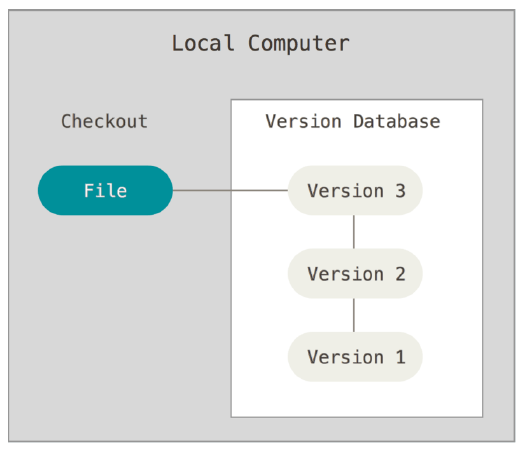
\includegraphics[scale=0.5]{LVC}  
	\caption[Local Version Control]{Local Version Control}
	\label{fig:LVC} 
\end{figure}

\subsubsection{Centralized Version Control System}
\textit{Local Version Control System} menjadi kurang efektif, bila ada beberapa orang yang berkolaborasi dengan pengembang. Karena pada \textit{Local Version Control System}, \textit{version control} dimiliki oleh masing-masing komputer sehingga pengguna tidak tahu apakah \textit{file} tersebut sudah diubah oleh kolaborator lain. CVCS(\textit{Centralized Version Control System}) memiliki sebuah \textit{server} yang menyimpan semua \textit{file} beserta historynya dan jumlah \textit{client} yang mengecek \textit{file} tersebut. Dengan adanya CVCS, semua orang mengetahui apa yang dilakukan oleh kolaborator yang mengerjakan proyek. Tetapi kelemahanya adalah ketika \textit{server} tersebut \textit{down}, tidak akan ada yang bisa berkolaborasi dan tidak dapat menyimpan perubahan yang sudah dikerjakan. Selain itu apabila data di \textit{server} tersebut hilang maka dan tidak melakukan \textit{back-up}, proyek yang sedang dikerjakan akan hilang beserta semua historinya. Struktur CVCS dapat dilihat pada Gambar~\ref{fig:CVCS}.

\begin{figure}[H]
	\centering  
	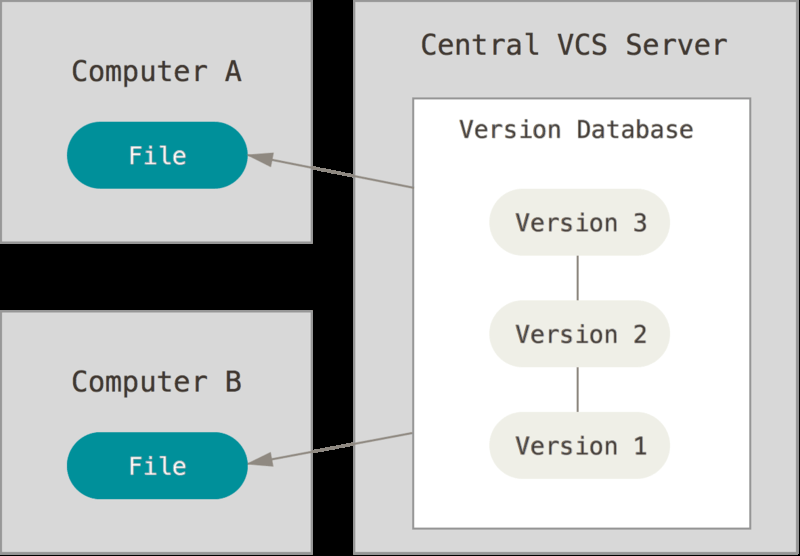
\includegraphics[scale=0.6]{CVCS}  
	\caption[Centralized Version Control]{Centralized Version Control}
	\label{fig:CVCS} 
\end{figure}

\subsubsection{Distributed Version Control System}
Dalam DVCS(\textit{Distributed Version Control System}) seperti \textit{Git, Mercurial, Bazaar dan Darcs}, \textit{client} tidak mengecek versi terbaru dari \textit{file} tetapi \textit{client} menggandakan \textit{repository} termasuk historinya. Jika \textit{server} mati/kehilangan data, maka \textit{client} memiliki \textit{file back-up} untuk mengembalikanya.  Ilustrasi DVCS terdapat pada Gambar~\ref{fig:DVCS}.

\begin{figure}[H]
	\centering  
	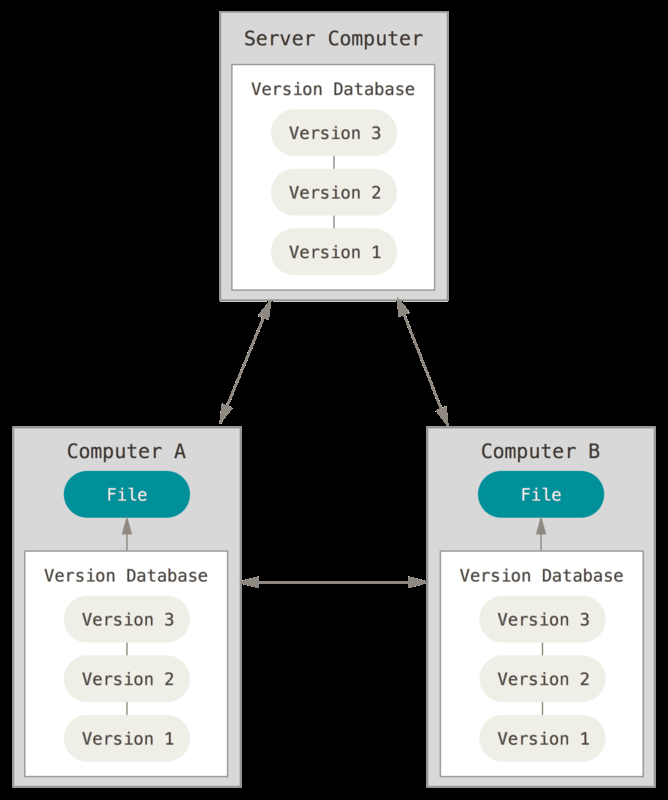
\includegraphics[scale=0.6]{DVCS}  
	\caption[Distributed Version Control]{Distributed Version Control}
	\label{fig:DVCS} 
\end{figure}

\subsection{\textit{Git}}
\textit{Git} merupakan sebuah \textit{version control} namun berbeda dengan VCS lainnya dilihat dari cara menyimpan datanya. Sistem seperti CVS, \textit{Subversion, Perforce, Bazzar} menyimpan data sebagai sekumpulan \textit{file} dan perubahan setiap \textit{file} disimpan setiap waktu. Pada \textit{Git}, data tersebut dianggap sebagai sekumpulan \textit{snapshot} dari \textit{miniature filesystem}. Setiap \textit{commit} atau menyimpan proyek, \textit{Git} seolah-olah mengambil gambar untuk melihat seperti apa \textit{file} yang terlihat pada saat itu dan menyimpannya sebagai referensi pada \textit{snapshot} tersebut. Singkatnya, apabila tidak ada \textit{file} yang diubah, Git tidak akan menyimpan \textit{file} lagi.\\

Hampir semua operasi pada \textit{Git} dapat dilakukan secara lokal. Ketika ingin menlihat histori suatu proyek, \textit{Git} akan mengambil data histori tersebut dari basis data lokal, sehingga tidak perlu memintanya ke \textit{server}. Selain itu, pengguna dapat bekerja secara \textit{offline}. Pada sistem lain seperti \textit{Perforce}, pengguna tidak dapat melakukan banyak hal jika tidak terkoneksi ke \textit{server} dan pada CVS, pengguna dapat mengubah \textit{file} tetapi tidak dapat \textit{commit} ke basis data. Pada \textit{Git}, pengguna dapat \textit{commit} dikarenakan \textit{Git} memiliki basis data lokal.\\

\textit{Git} memiliki 3 \textit{state} utama pada \textit{file} yaitu: 

\begin{itemize}
	\item \textit{committed} : data sudah tersimpan di basis data lokal.
	\item \textit{modified} : \textit{file} sudah diubah namun belum di\textit{commit} ke basis data.
	\item \textit{staged} : menandai file yang sudah dimodifikasi dalam versi sekarang untuk di\textit{commit}.
\end{itemize}

Terdapat 3 bagian utama dalam proyek \textit{Git} yaitu : 

\begin{itemize}
	\item \textit{Git directory} : tempat untuk menyimpan \textit{metadata} dan objek basis data untuk proyek yang dibuat. Ini adalah bagian terpenting dari \textit{Git} dan inilah yang di-\textit{copy} ketika \textit{clone repository} dari komputer lain.
	\item \textit{Working tree} : \textit{single checkout} sebuah versi dari proyek. \textit{File} diambil dari basis data yang sudah di\textit{compressed} di \textit{Git directory} dan disimpan pada \textit{disk} untuk digunakan dan dimodifikasi.
	\item \textit{Staging area} : sebuah \textit{file} yang ada di \textit{Git directory} yang menyimpan informasi tentang apa yang akan disimpan untuk \textit{commit} selanjutnya.  
\end{itemize}

Gambar~\ref{fig:gitState} di bawah ini menunjukan \textit{working tree, staging area dan Git directory}.

\begin{figure}[H]
	\centering  
	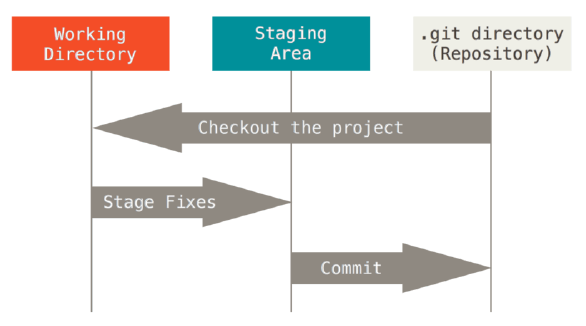
\includegraphics[scale=0.6]{gitState}  
	\caption[Working tree, staging area, dan Git directory]{Working tree, staging area, dan Git directory}
	\label{fig:gitState} 
\end{figure}

\textit{Workflow} pada \textit{Git} adalah sebagai berikut :

\begin{enumerate}
	\item Pengguna memodifikasi \textit{file} di \textit{working tree} milik pengguna.
	\item Pengguna memilih \textit{file} yang akan menjadi bagian dari \textit{commit} selanjutnya. \textit{File} yang terpilih akan ditambahkan ke \textit{staging area}. 
	\item Pengguna melakukan \textit{commit file} tersebut yang berada pada \textit{staging area} dan menyimpan \textit{snapshot} secara permanen ke \textit{Git directory}.
\end{enumerate}

Apabila versi tertentu dari sebuah \textit{file} sudah ada pada \textit{Git directory}, maka \textit{file} tersebut dalam berada dalam \textit{state committed}. Jika \textit{file} sudah dimodifikasi dan sudah ditambahkan ke \textit{staging area}, maka file tersebut dalam state \textit{staged}. Jika \textit{file} sudah diubah dan sudah di\textit{checkout} tetapi belum dalam \textit{state staged}, maka \textit{file} tersebut dalam \textit{state modified}.\\

Ada beberapa cara dalam menggunakan \textit{Git} yaitu dengan menggunakan \textit{command-line} dan beberapa GUI(\textit{Graphical User Interface}) yang memiliki kemampuan yang bermacam-macam. Pada umumnya digunakan \textit{command-line}, karena \textit{command-line} dapat menjalankan semua perintah \textit{Git} sedangkan GUI hanya memiliki sebagian fungsionalitas pada \textit{Git} supaya simpel dan mudah digunakan. 

\subsubsection{Mendapatkan \textit{Git Repository}}
Untuk mendapatkan \textit{Git repository} ada 2 cara yaitu : menjadikan sebuah proyek yang terdapat pada direktori lokal yang belum dalam \textit{version control} lalu menjadikannya sebagai \textit{Git repository} dan dengan \textit{clone Git repository} yang sudah ada.\\

Jika memiliki direktori proyek yang belum dalam \textit{version control} dan ingin mengontrolnya menggunakan \textit{Git}, hal pertama yang harus dilakukan adalah dengan membuka direktori proyek. Perintah untuk membuat repository pada \textit{Windows} adalah dengan mengetikan perintah \textit{\$ cd /c/user/my\_project} sesudah itu ketik perintah \textit{\$ git init}. Perintah tersebut akan membuat subdirektori bernama \textit{.git} yang mengandung semua repository yang dibutuhkan. Setelah mengetikan perintah di atas, proyek tersebut belum di-\textit{track} sama sekali. Untuk men-\textit{track file-file} pada sebuah proyek, pertama gunakan perintah \textit{git add} untuk men-\textit{track file} yang diinginkan kemudian ketik \textit{git commit} untuk commit file tersebut.\\

\textit{Clone repository} adalah mendapatkan \textit{copy} dari \textit{repository} yang sudah ada. Perintah yang digunakan adalah \textit{git clone}. Tidak hanya \textit{file-file} pada \textit{repository} saja yang di\textit{copy}, tetapi semua histori pada \textit{repository} tersebut akan ikut ter\textit{copy}. Perintah \textit{git clone} diikuti dengan \textit{url}. \textit{Url} ini berisi \textit{link} di mana \textit{repository} berada.

\subsubsection{\textit{Record} Perubahan pada \textit{Repository}}
Setiap \textit{file} dalam direktori memiliki 2 \textit{state} yaitu \textit{tracked} atau \textit{untracked}. \textit{Tracked file} adalah \textit{file} yang berada pada \textit{snapshot} terakhir. \textit{Tracked file} adalah \textit{file} yang \textit{Git} ketahui sekarang. \textit{Untracked file} adalah \textit{file} yang tidak berada pada \textit{snapshot} terakhir. Ketika \textit{file} diubah, \textit{Git} melihat bahwa \textit{file} tersebut sudah dimodifikasi, karena \textit{file} tersebut diubah setelah \textit{commit} terakhir. Kemudian \textit{file} yang sudah dimodifikasi tersebut di-\textit{stage} dan \textit{commit} semua \textit{file} yang sudah di\textit{staged} tersebut. Gambar~\ref{fig:lifecycle} menunjukan siklus hidup dari status \textit{file}.

\begin{figure}[H]
	\centering  
	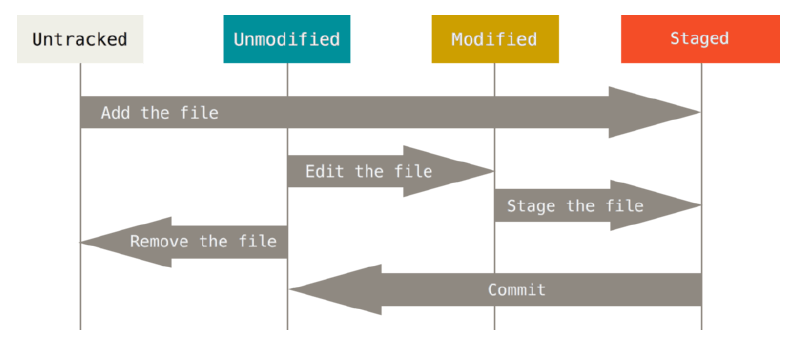
\includegraphics[scale=0.5]{lifecycle}  
	\caption[Siklus hidup pada status \textit{file}]{Siklus hidup pada status file}
	\label{fig:lifecycle} 
\end{figure}

Perintah \textit{git status} digunakan untuk mengecek status \textit{file}. Jika mengetik perintah sesudah \textit{clone}, maka tidak ada \textit{untracked file} karena pada saat \textit{clone}, tidak ada \textit{file} yang dimodifikasi. Bila menambahkan sebuah \textit{file} baru atau mengubah \textit{file} lalu mengetik perintah \textit{git status}, maka akan diberitahukan bahwa terdapat \textit{untracked file}. Karena itu untuk men-\textit{track file} baru, gunakan perintah \textit{git add} yang diikuti dengan nama \textit{file}nya seperti contoh ini : \textit{\$ git add README}. Perintah \textit{git add} tidak hanya digunakan untuk men-\textit{track file} baru. Selain digunakan untuk men-\textit{track file}, perintah \textit{git add} digunakan untuk stage \textit{file} yang sudah dimodifikasi.\\

Tidak semua \textit{file} akan ditambahkan secara otomatis oleh \textit{Git} atau ada \textit{file} yang ditunjukan sebagai \textit{file untracked}. Hal ini dapat diatasi dengan membuat sebuah \textit{file} yang bernama \textit{.gitignore}. \textit{File .gitignore} ini berisi \textit{file-file} yang tidak akan di-\textit{track} oleh \textit{Git}. \textit{File} yang biasanya ada dalam \textit{.gitignore} adalah \textit{log}, \textit{tmp} atau \textit{file} dokumentasi yang di\textit{generate} secara otomatis. Adapun aturan untuk \textit{pattern} yang dapat dimasukan pada \textit{file .gitignore} diantaranya adalah :

\begin{itemize}
	\item Baris kosong atau baris yang diawali dengan tanda pagar(\#) akan dibiarkan.
	\item \textit{Standard glob patterns}.
	\item \textit{Pattern} diawali dengan garis miring(/) untuk mencegah rekusrif.
	\item \textit{Pattern} diakhiri dengan garis miring untuk menspesifikasikan direktori.
	\item Menegasikan \textit{pattern} diawali dengan tanda seru(!).
\end{itemize}

\textit{Glob pattern} adalah \textit{regular expression} yang digunakan oleh \textit{shells}. Tanda bintang(*) untuk nol atau beberapa karakter, [abc] untuk karakter apa saja yang berada di dalam kurung siku, tanda tanya(?) untuk sebuah karakter apa saja dan tanda kurung siku dengan tanda strip(-) untuk karakter antara sebuah karakter dengan karakter lainya.\\

Perintah \textit{git commit} digunakan untuk \textit{commit file} yang sudah diubah dan ditambahkan. \textit{File} tersebut harus sudah di-\textit{stage} dengan menggunakan perintah \textit{git add}. \textit{File} yang belum di-\textit{stage} akan berada dalam state \textit{modified} meskipun sudah melakukan \textit{commit}. Untuk menambahkan keterangan tentang \textit{file} yang di\textit{commit} dapat dituliskan perintah \textit{git commit -m} yang diikuti dengan keterangan yang ingin disampaikan. 


\subsection{\textit{Git Branching}}
\textit{Branching} artinya membuat dan mengerjakan sebuah proyek di tempat yang berbeda namun masih dalam repository yang sama sehingga tidak mengubah proyek utama. Ketika \textit{commit}, \textit{Git} menyimpan objek \textit{commit} yang memiliki sebuah \textit{pointer} pada \textit{snapshot} sebuah konten yang sudah dalam \textit{state staged}. Objek ini mengandung nama pembuat dan alamat email, pesan yang diketik, dan \textit{pointer} ke \textit{commit}. \\

Misalkan seorang pengguna memiliki 3 \textit{file}, kemudian file tersebut semuanya di-\textit{stage} dan \textit{commit}. \textit{Staging file} akan mengkomputasi \textit{checksum} untuk setiap \textit{file}, menyimpan versi tersebut pada \textit{Git repository}(hal ini dapat disebut juga sebagai \textit{blobs}), dan menambah \textit{checksum} tersebut ke \textit{staging area}. Lalu \textit{Git} melakukan \textit{checksum} pada setiap \textit{subdirectory} dan menyimpan ketiga objek tersebut pada \textit{Git repository}. Sesudah itu \textit{Git} akan membuat objek \textit{commit} yang mengandung \textit{metadata} dan \textit{pointer} ke proyek \textit{root} sehingga dapat melihat \textit{snapshot} tersebut pada setiap versi. Sekarang, \textit{Git repository} memiliki 5 objek yaitu 3 \textit{blob} yang merepresentasikan 3 file, sebuah \textit{tree} yang mengandung isi direktori dan memberi nama \textit{blob} berdasarkan nama file yang di\textit{commit}, dan sebuah \textit{commit} dengan \textit{pointer} ke \textit{root tree} dan semua \textit{commit metadata}. Gambar~\ref{fig:branch} merupakan \textit{tree} dari penjelasan tersebut.

\begin{figure}[H]
	\centering  
	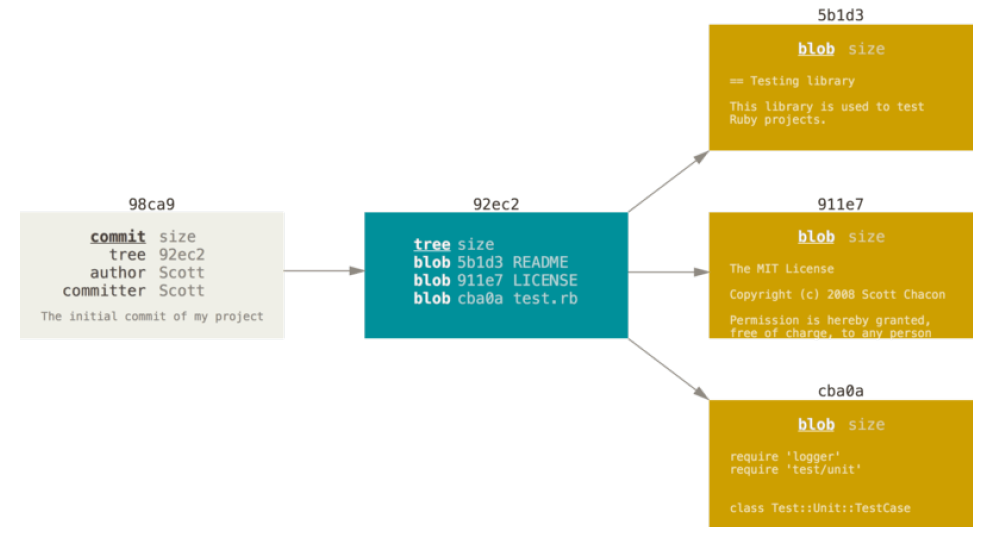
\includegraphics[scale=0.6]{branch}  
	\caption[Commit dan tree dari file yang dicommit]{Commit dan tree dari file yang dicommit}
	\label{fig:branch} 
\end{figure}

Jika ada perubahan pada proyek dan \textit{commit} proyek tersebut, maka \textit{commit} sesudahnya menyimpan \textit{pointer} pada \textit{commit} sebelum \textit{commit} terbaru seperti yang terdapat pada Gambar~\ref{fig:commitTree}. Jadi \textit{parent} dari sebuah \textit{commit} adalah \textit{commit} sebelumnya dan kemudian seterusnya.

\begin{figure}[H]
	\centering  
	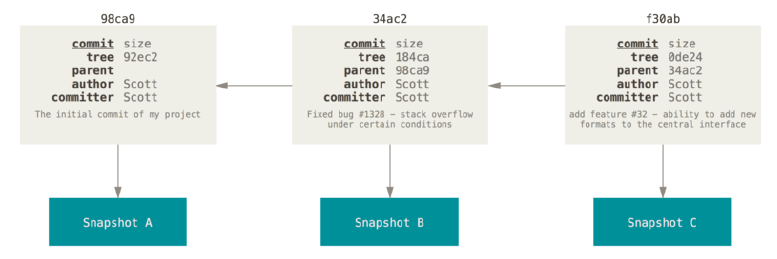
\includegraphics[scale=0.8]{commitTree}  
	\caption[Commit dan parent dari commit]{Commit dan parent dari commit}
	\label{fig:commitTree} 
\end{figure}

Nama \textit{branch} pada \textit{Git} awalnya disebut \textit{master}. Ketika \textit{commit}, pengguna diberikan \textit{branch master} yang menunjuk pada \textit{file} yang di\textit{commit} terakhir. Setiap \textit{commit}, pointer pada \textit{branch master} akan terus maju secara otomatis. 

\subsection{\textit{GitHub}}
\textit{GitHub} merupakan \textit{single host} terbesar untuk \textit{Git repository} dan sebagai titik tengah dari kolaborasi untuk jutaan pengembang dan proyek. Persentase terbesar dari semua \textit{Git repository} di\textit{hosting} di \textit{GitHub} dan banyak proyek \textit{open-source} menggunakanya untuk \textit{Git hosting, code review, issue tracking} dan lainnya. 

\subsubsection{\textit{Fork}}
Jika pengguna ingin berkontribusi pada proyek yang sudah ada dan pengguna tidak memiliki akses untuk \textit{push}, maka pengguna dapat \textit{fork} proyek tersebut. Ketika proyek tersebut telah di-\textit{fork}, \textit{GitHub} akan membuatkan sebuah \textit{copy/clone} dari proyek tersebut yang sekarang sudah menjadi milik penggunanya dan dapat di\textit{push}. Orang lain dapat \textit{fork} proyek, \textit{push} proyek, dan berkontribusi dalam perubahan tersebut kembali ke \textit{repository} aslinya dengan membuat \textit{Pull Request}.\\

Untuk \textit{fork} proyek, kunjungi halaman proyek dan klik tombol \textit{'Fork'} seperti pada Gambar~\ref{fig:forkButton} yang berada di atas kanan halaman. 

\begin{figure}[H]
	\centering  
	
\includegraphics[scale=1]{forkButton}  
	\caption[Tombol 'Fork']{Tombol 'Fork'}
	\label{fig:forkButton} 
\end{figure}

\textit{Github} didesain untuk \textit{collaboration workflow} tertentu yang berfokus pada \textit{Pull Request}. \textit{Flow} ini akan bekerja bila pengguna berkolaborasi dengan perusahhan yang \textit{globally-distributed} atau beberapa orang asing berkontribusi dalam sebuah proyek melalui banyak \textit{fork}. \textit{Flow}nya adalah sebagai berikut :

\begin{enumerate}
	\item \textit{Fork} proyek yang diinginkan.
	\item Buat topik \textit{branch} dari \textit{master}.
	\item Lakukan \textit{commit} untuk memperbaiki proyek.
	\item \textit{Push branch} ke proyek \textit{GitHub}.
	\item Buka \textit{Pull Request} di \textit{GitHub}.
	\item Diskusikan dan \textit{commit} proyek tersebut apabila proyek tersebut masih membutuhkan perbaikan.
	\item Pemilik proyek \textit{merges}/menggabungkan atau menutup \textit{Pull Requset}.
\end{enumerate}

\subsubsection{\textit{Pull Request}}
\textit{Pull Request} membuka tempat diskusi untuk \textit{owner(pemilik repository)} dan kontributor sehingga dapat berkomunikasi tentang perubahan tersebut sampai \textit{owner} merasa puas dan senang. Setelah itu \textit{owner} akan \textit{merge}/menggabungkan perubahan tersebut. Untuk membuat \textit{Pull Request}, bukalah halaman \textit{'Branches'} dan buat \textit{Pull Request} baru. Sesudah itu, akan muncul sebuah laman yang meminta mengisi judul dan deskripsi \textit{Pull Request} tersebut. Ketika tombol \textit{'Create pull request'} diklik,  maka pemilik proyek akan mendapatkan notifikasi bahwa seseorang menyarankan sebuah perubahan dan akan menghubungkan ke sebuah halaman yang memiliki semua informasi tersebut.\\ 

Setelah kontributor sudah membuat Pull Request, pemilik proyek dapat melihat saran  perubahan proyek dari orang lain, menggabungkan proyek, menolak perubahan proyek, dan memberikan komentar/keterangan pada perubahan tersebut. Sesudah pemilik proyek memberikan keterangan tentang perubahan tersebut, kontributor menjadi tahu apa yang harus dilakukan agar perubahan tersebut dapat disetujui. Apabila perubahan tersebut membuat pemilik proyek puas, pemilik proyek akan merge perubahan tersebut dengan proyek aslinya dan otomatis  akan menutup \textit{Pull Request}.